%!TEX root = ../Thesis.tex
%Chapter 1

\chapter{Symmetries of ($N\times N$) non-Hermitian Hamiltonian matrices}
\label{ChapterNNSymmetries}
\lhead{Chapter NxN. \emph{Symmetries of ($N\times N$) non-Hermitian Hamiltonian matrices}} % Write in your own chapter title to set the page header
%
A non-Abelian group of sixteen symmetry operations on (generally) \linebreak non-Hermitian
discrete Hamiltonians represented by $N\times N$ matrices is studied. The symmetry operations are described by unitary/antiunitary superoperators that arise  when combining
three basic generating operations with simple ``geometric'' interpretations. The corresponding Hamiltonian symmetries occur when
the Hamiltonian remains invariant under the superoperator action. These symmetries  include PT-symmetry and hermiticity as particular cases.
The interplay between the group of symmetry operations and Hamiltonian symmetries
is analyzed systematically by introducing the concepts of equivalent operations and associated symmetries.
Spectral properties implied by some of the symmetries are described.
%
\newpage
%
\section{Introduction}
%
Non Hermitian Hamiltonians have been used for a long time in nuclear, atomic, and molecular physics
as effective interactions, and have become common in optics, a field in which the wave equations in waveguides mimic  quantum Schr\"odinger equations \cite{Ruschhaupt2005,Longhi2017a,Konotop2016}.
%
Non Hermitian effective Hamiltonians may be constructed phenomenologically, in particular  to describe gain and loss, see e.g.
\cite{Ruschhaupt2005},
or be derived from a more fundamental Hermitian Hamiltonian
by projecting on a subspace \cite{Feshbach1958,Ruschhaupt2004a,Muga2004}.
%

In recent times PT-symmetric Hamiltonians \cite{Bender1998} have attracted much attention because of interesting and useful
spectral or scattering properties and many applications \cite{Longhi2017a,Konotop2016}, but recent work points at alternative symmetries \cite{Nixon2016,Nixon2016a,Chen2017,Ruschhaupt2017,Simon2018,Simon2019a} and even to a natural systematization of symmetry operations with a group structure  \cite{Ruschhaupt2017}. In \cite{Simon2019a} an abelian E8 group was described for symmetry operations on  ``scattering Hamiltonians''
that drive a particle state scattered off a potential center in one dimension (1D). It was shown there that devices for asymmetric response
forbidden by PT-symmetry, such as a  Maxwell demon,  are  compatible with some alternative symmetries. The present paper aims at extending the systematization
of symmetry operations to discrete and finite Hamiltonian matrices, for which a larger non-abelian group
of sixteen symmetry operations emerges naturally.

After reviewing briefly the results for scattering systems and pointing out the differences with discrete finite matrices
in the remaining part of the Introduction, we shall describe the symmetry operations by means of superoperators  in Sec. \ref{supo};
study the group of symmetry operations in Sec. \ref{groups};   its relation to actual Hamiltonian symmetries
 in Sec. \ref{collapse}; and spectral properties in Sec. \ref{sp}.
The paper ends with the conclusions and a discussion on open questions.
%
%
\subsection{Scattering Hamiltonians (review)}
%
%In this work we define the concept of symmetry like the invariance of an operator upon the action of a superoperator (will be defined better later). The core idea of this work is to analize a group of superoperators, their relations with themselves, their different group structures, the conditions that are needed to have equivalences (if the product of different superoperators upon the same operator are equal) and similar properties.
%
A strong motivation to study non-Hermitian, one-dimensional (1D) scattering Hamiltonians  $H=H_0+V$,\footnote{ $H_{0}=p^{2}/(2m)$ is the kinetic energy for a non relativistic particle of mass $m$,  $p$ being the momentum,  and $V$ is the potential, which is assumed to decay fast enough on both sides to have a continuous spectrum and scattering eigenfunctions}
is  the need to design devices with asymmetrical response,  ``asymmetrical devices" for short   \cite{Ruschhaupt2017},
for particles or waves incident from both sides, such as diodes, valves,  or rectifiers.
%one-way electronic devices
%(semiconductor materials doped with ``n"-type impurities in one half and with ``p"-type impurities in the other half)
%that let the electric current flow with little resistance one way while they obstruct the flow in the opposite way.
%These devices are useful to create transistors, which
%are the core of chips and computational technology.
%We also find  devices with asymmetrical response in nature, for example the valves of our circulatory system.
We may expect
%In view of the multiple and important applications of asymmetrical devices in the macroscopic world, it makes sense to assume that they will have
many applications of asymmetrical devices in optics or the microscopic world,
in quantum information processing  and other quantum technologies.

%Potentials with asymmetric response, i.e., such that  the transmission and reflection coefficients for incidence from the two sides of the potential
%have different values,  cannot be Hermitian, see e.g.  \cite{Ruschhaupt2017}.
%, we turn our attention to  non Hermitian ones.
%However, one can argue that due to the conservation of the probability, any real (meaningful) Hamiltonian should be Hermitian (the Hermiticity of the Hamiltonian is the property that imposes the conservation of the probability through time for a state descripted by that Hamiltonian). This is true, but it is a limitation only if you consider all the system (a close system) with the Hamiltonian. When we consider a subsystem, the probability to find a certain particle through the subsystem can be reduced (this probability can change, for example, from 1.0 to 0.9). This is possible because the probability is transfered from the subsystem to another part of the system (this can not happen in a close system, since by definition, it can not have exchanges of probability with the "exterior"). \cite{EPL}
%
%Like we have seen, this requirement of Hermiticity for the Hamiltonians it is not applicable to the study of an effective Hamiltonians for a subsystem. We can make an analogy with a circuit to understand how these potentials could help to create new quantum technology.
%
%If we compare an electronic circuit with a quantum system, the whole system Hamiltonian will be Hermitian, but our potential barrier will be a subsystem (therefore allowing it to be non Hermitian). The system would be the whole electric circuit and expressed by the whole Hamiltonian, while the subsystem would be a diode of the circuit and expressed by the non Hermitian effective Hamiltonian.
Ruschhaupt et al \cite{Ruschhaupt2017} describe  six types of  asymmetrical devices according to their transmission and reflection coefficients, and their relation,  in the form of selection rules,  to eight different symmetries that $H$ could fulfill
with the forms
%These symmetries are defined by one of the two equations
%
\begin{equation}
AH=HA, \label{commutation}
\end{equation}
%
\begin{equation}
AH=H^{\dagger}A, \label{pseudohermiticity}
\end{equation}
%
%
where $A$ is a unitary or antiunitary operator in the Klein four-group \linebreak $K_{4}=\lbrace 1,\Pi,\theta,\Pi\theta \rbrace$ \cite{Ruschhaupt2017}.
If (\ref{pseudohermiticity})  is fulfilled we say that $H$ is $A$-pseudohermitian \cite{Mostafazadeh2010,Ruschhaupt2017}.
The operators $\Pi$, $\theta$ and $\Pi\theta$ of the $K_{4}$ group are parity, time reversal (for a spinless particle) and the consecutive (commuting) application of both. Their properties are well known but we review them quickly for comparison with later,  different
usage of the symbols:

- $\Pi$: In the continuous space the parity operator is a linear, unitary  operator that inverts the position vector across the origin, so that
$\Pi c|x\rangle =c|-x\rangle$ for a complex number $c$. Also, $\Pi^2=1$.

- $\theta$: In the continuous space it is the ``temporal inversion'', an antilinear, antiunitary operator
%($\theta c |x \rangle =c^{*} |x\rangle $) that applied upon a ket changes its behavior in relation to time evolution,
%\footnote{For a time-independent  $H$ that commutes with $\theta$,
%the initial state at time $t=0$, $|\psi(0)\rangle$ is recovered as follows:  $\theta e^{-iHt/\hbar} \theta |\psi(t)\rangle=\theta e^{-iHt/\hbar} \theta e^{-iHt/\hbar}|\psi(0)\rangle=\theta e^{-iHt/\hbar}  e^{iHt/\hbar}\theta|\psi(0)\rangle=|\psi(0)\rangle$.
%Instead, in general,  if $H$ does not commute with $\theta$, $\theta e^{-iH_\theta t/\hbar} \theta |\psi(t)\rangle=\theta e^{-iH_\theta t/\hbar} \theta e^{-iHt/\hbar}|\psi(0)\rangle=\theta e^{-iH_\theta t/\hbar}  e^{iH_\theta t/\hbar}\theta|\psi(0)\rangle=|\psi(0)\rangle$, where
%$H_\theta=\theta H\theta$.  ``Forwards'' and ``backwards'' motions depend on different Hamiltonians: $H$ and $H_\theta$.}
that on a spinless-particle state acts  in coordinate and momentum representations as follows,
%
\begin{equation}
\label{int1}
\theta \int dx |x\rangle\langle x|\psi\rangle = \int dx |x\rangle\langle \psi|x\rangle,
\end{equation}
%
\begin{equation}
\label{int2}
\theta \int dp |p\rangle\langle p|\psi\rangle = \int dp |-p\rangle\langle \psi |p \rangle,
\end{equation}
%
so that $\theta\theta=1$.

- $\Pi\theta$:  It is also antilinear
and antiunitary
since the product of a linear operator and an antilinear operator is antilinear.
$\Pi$ and $\theta$  commute. It is also often called ``$PT$''.

Combining  the two possible relations (\ref{commutation}) and (\ref{pseudohermiticity}), and the four $A$ in  Klein's group, we get the  eight symmetries in \cite{Ruschhaupt2017}
made explicit in table \ref{table11}, column iii. They may be regarded as the invariance of the Hamiltonian with respect to
corresponding eight symmetry operations that form the abelian group E8 \cite{Simon2019a},
see column ii.

Let us emphasize and insist on the  important distinction between  {\it symmetry operations}  on and {\it symmetries} of an operator or of the corresponding matrix. Symmetry operations are changes imposed  to an operator or matrix,  e.g. transformations such as  taking the complex conjugate, or performing  the transpose. An operator or matrix possesses a particular symmetry if the corresponding symmetry operation keeps the operator or matrix {\it invariant}. The roman number  code in column i  of table \ref{table11} will refer indistinctly to an  operation or to a symmetry,  the context should clarify the possible ambiguity.



%The relation between the eight symmetries and the different device types is shown in table \ref{table12}, see \cite{Ruschhaupt2017} for further details.
%
%
%
\begin{table}[t]
\caption{
{i}) Roman number code that may represent the operation or the symmetry.
{ii}) Result of performing eight symmetry operations on $H$.
 {iii}) Corresponding symmetries of the types (\ref{commutation}) or (\ref{pseudohermiticity}).
When $H$ is invariant under the operation, the matrix elements of $H$ obey these relations, and viceversa.
 }
\label{table11}
\begin{tabular}{ lll }
%  \hline
%  \multicolumn{5}{l} \\
%  \mr
  i&ii&iii\\
  \hline
%  \multicolumn{3}{l}{Symmetries considering the Klein 4-group} \\
%  \mr
   I     &     $H$                               &$\langle x|H|y \rangle=\langle x|H|y \rangle$                  \\
   II    &     $H^{\dagger}$                  & $\langle x|H|y \rangle=\langle y|H|x \rangle^{*}$         \\
   III   &     $\Pi H\Pi $                     & $\langle x|H|y \rangle=\langle -x|H|-y \rangle$               \\
   IV    &    $\Pi H^{\dagger}\Pi$         & $\langle x|H|y \rangle=\langle -y|H|-x \rangle^{*}$      \\
   V     &    $\theta H\theta$               & $\langle x|H|y \rangle=\langle x|H|y \rangle^{*}$         \\
   VI    &    $\theta H^{\dagger}\theta$        & $\langle x|H|y \rangle=\langle y|H|x \rangle$     \\
   VII   &    $\Pi\theta H\Pi\theta$    & $\langle x|H|y \rangle=\langle -x|H|-y \rangle^{*}$         \\
   VIII  &    $\Pi\theta H^{\dagger}\Pi\theta$ & $\langle x|H|y \rangle=\langle -y|H|-x \rangle$.\\


\end{tabular}

\end{table}
%
%

As pointed out first for Hamiltonians with discrete spectrum by A. Mostafazadeh \cite{Mostafazadeh2002,Mostafazadeh2002a,Mostafazadeh2002b} and later extended to scattering
Hamiltonians in \cite{Simon2019a}, \linebreak $A$-pseudohermiticity with $A$ linear, or the commutation of $A$ and $H$ for $A$ antilinear
imply that the eigenvalues of $H$ come in conjugate pairs necessarily, in particular they
may be real.
These conditions occur for symmetries II, IV, V, and VII.
No other symmetry in this set of eight or in the extension to sixteen symmetries
considered below satisfies them.





%

%We know that $H_{o}$ has certain properties, like for example its Hermiticity. This is a clear limitation of the possible symmetries of H (like we will see bellow), and for that reason we have only considered the eight symmetries above. We can see that the Hermiticity is one of those symmetries, but it does not produce any assymetrical response.
%
%
%
\subsection{$N\times N$ Hamiltonian matrices}
%
%
The above analysis has to be extended when dealing with
discrete Hamiltonians represented by $N\times N$ finite matrices in some orthonormal basis, such as the ones used to describe 2-level, 3-level, or N-level systems in simplified models of atomic structure or of artificial atoms in solid state physics or in optics.
In this work it is assumed that  the  discrete Hamiltonians \footnote{By default a  ``discrete'' basis or matrix is always  finite here.} are diagonalizable,
%
\begin{equation}
H=\sum_{i} |\phi_{i}\rangle E_{i}\langle\widehat{\phi_{i}}|,
\end{equation}
%
where the right, $|\phi_{i}\rangle$, and left eigenvectors, $\langle \widehat{\phi_{i}}|$, are biorthogonal partners, and $E_i$ may be a complex number.
These vectors  form a biorthogonal basis such that  $1=\sum_i |\phi_{i}\rangle \langle\widehat{\phi_{i}}|$
and $\langle\widehat{\phi_{i}}|\phi_{j}\rangle=\delta_{ij}$.


To study the possible  symmetries and symmetry operations for discrete Hamiltonians we shall first reset  the meaning of the operators $\Pi$, $\theta$, and $\Pi\theta$ to adapt them to a discrete  orthonormal basis.
%We will not use them as the usual parity, inverting the space,  and time reversal, inverting the time.
They will stand now  as ``geometrical" operators in a given basis as follows (more on this geometrical aspect in Sec. \ref{gi}
below):


- $\Pi$: For a finite orthonormal basis with basis states $|1\rangle, |2\rangle, ...,|N\rangle$,
labeled by  natural numbers, it transforms (linearly) the $i$-th member of the basis to $-i$, $\Pi c|i\rangle =c|-i\rangle $, where $-i$ implies the ``opposite'' of $i$ with respect to  the middle
value of the basis index, i.e.,
%
\begin{equation}
|-i\rangle\equiv|N+1-i\rangle.
\end{equation}
%
Example: for a  basis $\lbrace |1\rangle ,|2\rangle ,|3\rangle  \rbrace$, $N=3$ so $|-1\rangle =|3\rangle $,$|-3\rangle =|1\rangle $, and $|-2\rangle =|2\rangle $. (A basis could also have an even number of states and a half-integer middle value.) $\Pi$  is a unitary operator.  We may also regard it as a ``reflection'' operator.
%We can call this a ``geometrical" transformation of the matrix.



- $\theta$: In the discrete basis, it will be an antilinear, antiunitary  operator defined by  $\theta c |j\rangle =c^{*} \theta |j\rangle =c^{*}|j\rangle $, where $c$ is any complex constant.



- $\Pi\theta=\theta\Pi$:  It is antilinear and antiunitary.



Note that in both discrete and continuous models, the operators $\Pi$, $\theta$, and $\Pi\theta$ are their own inverses, and also Hermitian operators.
%Furthermore, $\Pi$ is unitary and $\theta$ and $\Pi\theta$ antiunitary.

Since the structure of a discrete Hamiltonian does not have the limitations imposed by the properties of the kinetic energy Hamiltonian $H_{0}$ in the scattering form $H=H_{0}+V$,
a larger group of sixteen symmetry operations that could leave the Hamiltonian invariant
is found compared to the
symmetry operations on scattering Hamiltonians, see table \ref{table31}.
% is a compendium of the symmetry operations expressed with different notations.
%In addition to the eight symmetry operations that
%
%
%. We will limit ourselves to the non relativistic case in 1D, so $H_0=p^{2}/2m=-\frac{\hbar^{2}}{2m}\frac{\partial^2}{\partial x^2}$. The symmetries forbidden by $H_{0}$ are the ones shown in  Table \ref{tab:00} that are not of the types .
The  new operations with respect to those in  table 1, from $IX$ to $XVI$, imply to  invert  one of the kets but not the other one, applying parity only on one side. The corresponding symmetries do not have the forms (\ref{commutation}) or (\ref{pseudohermiticity}).



%%($\langle x'| H_{0}|x\rangle =-\hbar^2/(2m)\delta(x-x')\partial^2/\partial  x^2$  cannot be %%invariant upon them).
%some of these transformations, specifically from $IX$ to $XVI$, which are not of the type (\ref{commutation}) or (\ref{pseudohermiticity}).
%The kinetic energy


\hspace*{-1cm}
\begin{table}
\hspace*{-1cm}
\caption{{Group elements (transformations) in different notations}. 1: Roman number code; 2: Group theory notation of group elements in terms of generators $x$, $y$, $a$, see (\ref{18}) and (\ref{19}); 3: Superoperators ${\cal S}$;
4: Explicit action of the superoperators on $H$; 5: Geometrical interpretation of the symmetry operations, where --- is the horizontal axis, $\mid$ the vertical axis, $\setminus$ is the main diagonal,
$/$ is the secondary diagonal, and cc is complex conjugation;
 6: Matrix element $\langle i |({\cal S}H)| j \rangle$. A Hamiltonian symmetry occurs if $\langle i |({\cal S}H)| j \rangle=\langle i |H| j \rangle$ for all $i, j$.\label{table31}}

\begin{tabular}{llllll}
%  \multicolumn{5}{l} \\
%  \mr
  1&2&3&4&5&6\\
  \hline
  I&$e$           & ${\cal{L}}_{1}$&$H$ &do nothing&$\langle i|H| j\rangle$ \\
  II&$x$           & ${\cal{D}}$&$H^\dagger$&flip along $\setminus$ and cc&$\langle j|H| i\rangle^*$  \\
  III&$a^{2}$     & ${\cal{L}}_{\Pi}$&$\Pi H\Pi$&rotate by $\pi$&$\langle -i|H| -j\rangle$ \\
   IV&$x a^{2}$   & ${\cal{L}}_{\Pi}{\cal{D}}$&$\Pi H^\dagger \Pi$&flip along $/$ and cc &$\langle -j|H| -i\rangle^*$ \\
  V&$y$           & ${\cal{L}}_{\theta}$&$\theta H\theta$&cc&$\langle i|H| j\rangle^*$ \\
  VI&$xy$          & ${\cal{L}}_{\theta}{\cal{D}}$&$\theta H^\dagger \theta$&flip
  along $\setminus $   &$\langle j|H| i\rangle$ \\
    VII&$a^{2}y$    & ${\cal{L}}_{\Pi\theta}$&$\Pi\theta H\Pi\theta$&rotate by $\pi$ and cc&$\langle -i|H| -j\rangle^*$ \\
  VIII&$a^{2}xy$   & ${\cal{L}}_{\Pi\theta}{\cal{D}}$&$\Pi\theta H^\dagger\Pi\theta$&flip along $/$ &$\langle -j|H| -i\rangle$ \\
    IX&$ax=xa^{3}$ & ${\cal{L}}_{1,\Pi}$&$H\Pi$&flip along $\mid$ &$\langle i|H| -j\rangle$ \\
  X&$xa=a^{3}x$ & ${\cal{L}}_{\Pi,1}$&$\Pi H$&flip along --- &$\langle -i|H| j\rangle$ \\
  XI&$axy$         & ${\cal{L}}_{\theta}{\cal{L}}_{1,\Pi}$&$\theta H\theta\Pi$&flip along $|$ and cc&$\langle i|H| -j\rangle^*$ \\
  XII&$a^{3}xy$   & ${\cal{L}}_{\theta}{\cal{L}}_{\Pi,1}$&$\Pi\theta H\theta$&flip along --- and cc&$\langle -i|H| j\rangle^*$ \\
 XIII&$a$           & ${\cal{L}}_{1,\Pi}{\cal{D}}$&$H^\dagger\Pi$&rotate by $\pi/2$ and cc&$\langle -j|H| i\rangle^*$ \\
 XIV&$a^{3}$     & ${\cal{L}}_{\Pi,1}{\cal{D}}$&$\Pi H^\dagger$&rotate by $3\pi/2$ and cc&$\langle j|H| -i\rangle^*$ \\
 XV&$ay=ya$     & ${\cal{L}}_{\theta}{\cal{L}}_{1,\Pi}{\cal{D}}$&$\theta H^\dagger \Pi\theta$&rotate by $\pi/2$ &$\langle -j|H| i\rangle$ \\
  XVI&$a^{3}y$    & ${\cal{L}}_{\theta}{\cal{L}}_{\Pi,1}{\cal{D}}$&$\theta\Pi H^\dagger \theta$&rotate by $3\pi/2$&$\langle j|H| -i\rangle$\\
\end{tabular}

\end{table}
%





%\clearpage





%Note that the conditions $XV$ and $XVI$ in the right  column of table \ref{tab:00} carry the same meaningful symmetry,  in the sense that they imply each other, and this also happens with XIII and XIV. However, the corresponding symmetry operations (represented in the second column) are distinct.  The proof of these associations will be done in the Section \ref{secx}, where
%we shall discuss in more detail equivalent and associated symmetry operations.

This work is devoted to study the group of 16 symmetry operations and their relations with actual Hamiltonian symmetries.
Before discussing properties of the abstract group we shall introduce its  realization based on superoperators and their geometrical interpretation.
%
%
%
%
%
%
%
\section{Superoperators\label{supo}}
%
%
%
%
%
%Superoperators play a key role here  as they will represent the symmetry operations.
%The concept  of symmetry followed in this work  is compactly expressed by ``change without changing'' \cite{Wilczek2015}, namely,
%there is a symmetry when an  operation (change) on some object leaves it invariant. %This is a fundamental idea in all branches of Physics with  powerful consequences.
%In our context the object is the Hamiltonian, and the changes are expressed
%by superoperators.
%A  Hamiltonian $H$ will have a certain symmetry if it is invariant upon the action of a  superoperator.
%All operators are invariant upon at least one superoperator, the identity.
Different superoperator types are used in the group of sixteen in table \ref{table31}.

Let us define first  superoperators ${\cal L}_{A,B}$ by  left multiplying  by $A$ and right multiplying by
$B$,
%
\begin{equation}
{\cal{L}}_{A,B}H=AHB.
\end{equation}
%
Note that ${\cal{L}}_{A,B}H=H \iff A^{-1}H=HB$.
%
We consider only ${\cal{L}}_{A,B}$ where both $A$ and $B$ are  linear or both are antilinear, so as to preserve the linearity of a Hamiltonian. Otherwise ${\cal{L}}_{A,B}$ could not represent a symmetry. For example, the superoperator ${\cal{L}}_{1,\theta}$ creates an antilinear operator ${\cal{L}}_{1,\theta}H=H\theta$, so it is not in the  group of sixteen transformations.
The operators $A$, $B$ to construct  the  superoperator group will be chosen among  Klein's group operators
1, $\Pi$, $\theta$, and $\theta\Pi$, defined for a finite basis.

A shorthand notation ${\cal{L}}_{A}$ is  used for ${\cal{L}}_{A^{-1},A}$,
%
\begin{equation}
{\cal{L}}_{A}H=A^{-1}HA,
\end{equation}
%
where $A^{-1}$ is the inverse of $A$.
It is easily seen that  ${\cal{L}}_{A}H=H \iff [H,A]=0.$

To complete the sixteen operations we also define a ``dagger'' superoperator ${\cal{D}}$ that transforms an operator  into its adjoint \cite{Simon2018},
%
\begin{equation}
{\cal{D}}H=H^{\dagger}.
\end{equation}
%
%\begin{small}
{Hermiticity is  the symmetry that corresponds to invariance upon this superoperator.}
%\end{small}
%

It is possible to combine the former superoperators applying them sequentially to find new ones \cite{Simon2018},
for example,
%
\begin{equation}
{\cal{L}}_{A}{\cal{D}}H=A^{-1}H^{\dagger}A,
\end{equation}
\begin{equation}
{\cal{D}}{\cal{L}}_{A}H=(A^{-1}HA)^{\dagger}.
\end{equation}
%
%\begin{small}
${\cal{L}}_{A}{\cal{D}}H=H\iff AH=H^\dagger A$.
{In general  ${\cal{L}}_{A}{\cal{D}}H \neq {\cal{D}}{\cal{L}}_{A}H $, but ${\cal{L}}_{A}$ and ${\cal{D}}$   commute when $A^{-1}=A^{\dagger}$, as it happens for our basic operators $1$, $\Pi$, $\theta$ and $\theta\Pi$ in Klein's group.



%\end{small}


%If in addition  we  use ${\cal{L}}_{\dagger}$,
%This means hermiticity is a symmetry in our study, on the same footing as all the rest.
%\clearpage
The group of superoperators that preserve linearity are given in columns 3 and 4 of table \ref{table31}.
%, compare to  table \ref{table11}.
A sense of  ``completeness'' of the sixteen operations is discussed below in Sec. \ref{gi} from a geometrical perspective.
%, without the limitations of the $H=H_{0}+V$ structure.
As before the roman numbers in column 1 are conventional indices for operations and/or symmetries, and when the matrix element in the rightmost column 6 equals $\langle i|H|j\rangle$,
$H$ is invariant under the transformation and posseses a symmetry.
It proves convenient to denote an arbitrary superoperator in this group by a generic notation ${\cal S}$.
In formal manipulations we shall later on use distinguishing subscripts, e.g.  ${\cal S}_j$, where $j=1, 2,...,16$ mapping $I\to 1$, $II\to2$, etc...


Superoperators,  just like ordinary operators,  are linear if they leave complex constants invariant and antilinear if they transform them to their complex conjugates.
In particular  \cite{Simon2018},
%
%
\begin{eqnarray}
{\cal{L}}_A (c H)&=& c A^\dagger  H A,\;\;\,  A\, {\rm unitary},
\nonumber\\
{\cal L}_A (c H)&=& c^* A^\dagger  H A,\;  A\, {\rm antiunitary},
\nonumber\\
{\cal{L}}_{A,B} (c H)&=& c A  H B,\;\;\,  A\, and \ B \ {\rm unitary},
\nonumber\\
{\cal{L}}_{A,B} (c H)&=& c^{*} A  H B,\;\;\,  A\, and \ B \ {\rm antiunitary},
\nonumber\\
{\cal D} (c H)&=& c^*H^\dagger,
\nonumber\\
%{\cal L}_{A,\dagger} (c H)&=&
{\cal L}_A  {\cal D} (cH)&=&{\cal D} {\cal L}_A  (cH)=c^* A^\dagger H^\dagger A,\;
A\, {\rm{unitary}},
\nonumber\\
%{\cal L}_{A,\dagger} (c H)&=&
{\cal L}_A  {\cal D} (cH)&=&{\cal D} {\cal L}_A  (cH)= c A^\dagger H^\dagger A,
A\, {\rm{antiunitary}}.
\end{eqnarray}
%


\subsubsection{Valid symmetry operations.\label{sst}}
%

%This concept embraces more symmetries than the ones expressed by the commutation of a unitary or antiunitary operator with $H$, see Eq. (\ref{commutation}).
%Actually, because of the possibility to include  ${\cal{L}}_{A,B}$ superoperators as valid symmetry transformations  for discrete Hamiltonians, we deal with
%sixteen symmetry transformations rather than the eight ones studied in  \cite{Simon2018}.
%%In \cite{Ruschhaupt2017} the concept of symmetry was extended beyond $[A,H]=0$ to include $A$-pseudohermiticiy, see Eq. (\ref{pseudohermiticity}). In this paper we consider a broad physical scenario
%%(any system describable by discrete Hamiltonians) where the possible symmetries go even beyond
%%these two types.
%We will show how by superoperators both conmutation and A-pseudohermiticity can be described (we will only consider linear or antilinear operators as A):

The transformations considered in quantum physics as possible symmetries, i.e. symmetry transformations (operations), are not really arbitrary. Wigner set the rule that they should leave the modulus of the  scalar product of two states, equivalently their ``transition probability'', invariant,  and this restricts the corresponding operators to be unitary or antiunitary \cite{Wigner1959}. As seen below in detail, our  superoperators imply a mild generalization of Wigner's definition, as they  leave the scalar product of two
density operators, which constitute the most general way of expressing a state, invariant.

%Symmetries of the form $[H,A]=0$ correspond to the invariance upon the superoperator ${\cal{L}}_{A}H=A^{-1}HA$, since
%
%\begin{equation}
%{\cal{L}}_{A}H=A^{-1}HA=H \ {\rm if} \ [H,A]=0,
%\end{equation}
%
%and, in reverse, if ${\cal{L}}_{A}H=H$,
%\begin{equation}
%A[A^{-1}HA=H] \Rightarrow HA=AH \Rightarrow [A,H]=0.
%\end{equation}
%
%Similarly, $A$-pseudohermiticity corresponds to invariance with respect to the superoperator ${\cal{L}}_{A}{\cal{L}}_{\dagger}$.
%
%If $AH=H^{\dagger}A$,
%
%\begin{equation}
%H={\cal{L}}_{A}{\cal{L}}_{\dagger}H=A^{-1}H^{\dagger}A.
%\end{equation}
%In reverse, if ${\cal{L}}_{A}{\cal{L}}_{\dagger}H=H$,
%\begin{equation}
%A[H=A^{-1}H^{\dagger}A]\Rightarrow AH=H^{\dagger}A.
%\end{equation}
%
%Also, if $A^{-1}H=HB$,
%
%\begin{equation}
%{\cal{L}}_{A,B}H=AHB=H,
%\end{equation}
%and, in reverse, if ${\cal{L}}_{A,B}H=H$,
%\begin{equation}
%A^{-1}[H=AHB]\Rightarrow A^{-1}H=HB.
%\end{equation}
%
%
%\subsection{Properties of the superoperators and their relation to the scalar product}
%
%

%Continuing with the analogy between the relations of the operators with the states and the superoperators with the operators,
%we will now  define the scalar product of two operators, the effect of the superoperators on them, and, thanks to that, the adjoint of a given superoperator.



We will denote a scalar product of two given (linear) operators $F$ and $G$ as $ \langle\langle F,G \rangle\rangle$. The general expression of the scalar product of two linear operators is $\langle\langle F,G \rangle\rangle=Tr(F^{\dagger}G)$ \cite{Simon2018}. Expectation values for an observable $F$ and a density operator $\rho$, both hermitian, take the form $\langle F\rangle=Tr[F\rho]=Tr[F^{\dagger}\rho]=\langle\langle F,\rho \rangle\rangle$.

Now, we can define the adjoint of a given superoperator ${\cal{S}}$ as the superoperator ${\cal{S}}^\dagger$ which fulfills  \cite{Simon2018}
%
\begin{equation}
\langle\langle G,{\cal{S}}F\rangle\rangle=\langle\langle F,{\cal{S}}^{\dagger}G\rangle\rangle^{*} \, \ {\rm for \ {\cal{S}} \ linear},
\end{equation}
\begin{equation}
\langle\langle G,{\cal{S}}F\rangle\rangle=\langle\langle F,{\cal{S}}^{\dagger}G\rangle\rangle \, \ {\rm for \ {\cal{S}} \ antilinear}.
\end{equation}
%
%In these expressions we will always assume that the superoperator is applied upon a linear operator (such as the Hamiltonian or the density operator).
For   unitary or antiunitary operators $A$, so $A^{-1}=A^{\dagger}$, we find  \cite{Simon2018}
%
\begin{eqnarray}
{\cal L}_A^\dagger(\cdot)&=& {\cal L}_{A^\dagger}(\cdot)\equiv A(\cdot)A^\dagger,
\nonumber\\
%\end{equation}
%\begin{equation}
{\cal D}^\dagger(\cdot) &=&{\cal D}(\cdot),
%\end{equation}
%\begin{equation}
\nonumber\\
({\cal L}_{A}{\cal D})^\dagger (\cdot) &=& {\cal L}_{A^\dagger}{\cal D}(\cdot)\,.
\label{adj}
\end{eqnarray}
%
For  a more general ${\cal{L}}_{A,B}$, with $A$ and $B$ both unitary or aniunitary,
${\cal{L}}_{A,B}^{\dagger}={\cal{L}}_{A^{\dagger}B^{\dagger}}$. This is easy to check
when $A$ and $B$ are both unitary,
%
\begin{eqnarray}
&&\langle\langle F,{\cal L}_{A,B}^{\dagger}G \rangle\rangle= \langle\langle G,{\cal L}_{A,B}F \rangle\rangle^{*}
\nonumber\\
&=&Tr[(G^{\dagger}AFB)^\dagger] = Tr[B^{\dagger}F^\dagger A^\dagger G]
\nonumber\\
&=&Tr[F^{\dagger}A^\dagger G B^\dagger],\, {\rm using \ cyclic \ permutation.}
\end{eqnarray}
%
For antiunitary $A$ and $B$, ${\cal{L}}_{A,B}$ is antiunitary and the calculation is more elaborate  but the result is the same.
%The proof when they result also holds when both $A$ and $B$ V is more detailed operators $A$ and $B$ may be also antilinear, in this work $\theta$ or $\Pi\theta$. If $A=B$, then   ${\cal{L}}_{A,B}={\cal L}_{A}$, and if $A \neq B$, we could decompose the superoperator in two like ${\cal L}_{1,\Pi}{\cal L}_{\theta}$ or ${\cal L}_{\Pi, 1}{\cal L}_{\theta}$, whose adjoints have been discussed.



For all sixteen superoperators an explicit calculation gives  ${\cal{S}}^{\dagger}={\cal{S}}^{-1}$, so these superoperators are  unitary or antiunitary. This is clear in the set (\ref{adj}) and  for ${\cal{L}}_{A,B}$ it  is also true because we only consider $A$ and $B$ to be simultaneously unitary or antiunitary. Thus  ${\cal{L}}_{A,B}{\cal{L}}_{A^{\dagger}B^{\dagger}}F=AA^{\dagger}FB^{\dagger}B=F$,
and similarly ${\cal{L}}_{A^{\dagger}B^{\dagger}}{\cal{L}}_{A,B}F=F$.


Parallel to the fact that a unitary or antiunitary operator $A$ keeps the scalar product of two states represented by kets invariant ($|\psi_{1}\rangle,|\psi_{2}\rangle \Rightarrow \langle\psi_{1}|\psi_{2}\rangle$ ;\linebreak $A|\psi_{1}\rangle,A|\psi_{2}\rangle \Rightarrow \langle\psi_{1}|A^{\dagger}A|\psi_{2}\rangle=\langle\psi_{1}|\psi_{2}\rangle$), unitary and antiunitary superoperators keep  invariant the scalar product of two density operators,
%
\begin{equation}
\langle\langle \rho_{1},\rho_{2}\rangle\rangle=\langle\langle {\cal{S}}\rho_{1},{\cal{S}}\rho_{2} \rangle\rangle.
\end{equation}
%
This property defines, extending Wigner's approach to symmetry \cite{Zee2016}, a symmetry transformation.

%\subsubsection{Explicit group of superoperators.}

%Once we have a general definition of the superoperator concept, we can start by explaining which will be the superoperators we will analize (but the fact that we do not use more superoperators does not mean that their are not, but that we think these are the most usefull ones).


%gives the conditions that the matrix of $H$ must obey to be invariant upon the superoperator.

%Considering these basic operations for discrete Hamiltonians we can create sixteen symmetries and
%corresponding symmetry operations.
% with 14 meaningful symmetries for the Hamiltonian.
%Eight of the symmetries are similar to the ones we had for scattering systems using  the group $K_{4}$ combined with  (\ref{commutation}) and (\ref{pseudohermiticity}), but with
%discrete kets $|i\rangle$ instead of continuous ones $|x\rangle$.
%Table \ref{table31}, column 6, depicts the conditions that the matrix components of the Hamiltonian should obey if the symmetry operation leaves the matrix invariant,  in which case it represents a symmetry of the Hamiltonian.
%The reader may notice that some combinations are not present in the list of sixteen operations, see column 4 in table
%\ref{table31},
%for example there is no $\theta H$  because  $H$ is a linear operator and the result
%would be antilinear, so acting with $\theta$ only on one side  cannot lead to a Hamiltonian symmetry.


%\clearpage


%
%
%
\section{Study of the group \label{groups}}
%
%
%
The set of 16 superoperators (symmetry operations)  has a group structure, it may be considered as the direct product of the dihedral group D8 and the cyclic group Z2 and has many subgroups that we shall briefly discuss. To the best of our knowledge the group is not known by any particular name, so we shall  call it $G_{16}$ for short.
The abstract group in our case is realized by all transformations that can be performed on a discrete Hamiltonian matrix making use of complex conjugation, transposition, and inversion of one or two states in the matrix element. This is a group of {\it symmetry operations} on the Hamiltonian matrices, not necessarily the group of symmetries of a given Hamiltonian.
%If the transformation leaves the matrix invariant, then it is a symmetry of the Hamiltonian. %We shall see that some Hamiltonian symmetries are strongly related to each other, in the sense that if some symmetries occur then others are automatically satisfied and viceversa.
%This group of order 16 has  many subgroups that we will discuss below.

%
%
%
\subsection{Structure of the group.}
%
%
%
%Like any group, this one has a certain structure with interesting properties. It has also interesting subgroups, for example two elementary-abelian E8 type groups. One of them has been studied intensively to represent transformations on  non Hermitian scattering Hamiltonians \cite{Ruschhaupt2017,Simon2019a}.



%We  notice that certain members (superoperators) of the group conmute with each other, but others do not.
%reminiscent of the symmetry operators of different order  in fields like crystalography (where we find rotations or symmetry planes of different orders, like we have operators of different orders).
%
%
\subsubsection{Group of 16 transformations.}
%
%
$G_{16}$ is not abelian. Not all the elements of the group
commute with each other, even thought some of them do.
We also notice that most of the elements are their own inverses, except XIII, XIV, XV, and XVI.
Their inverse is the application of themselves 3 times,  $({\cal{L}}_{1,\Pi}{\cal{D}})^{-1}=({\cal{L}}_{1,\Pi}{\cal{D}})^{3}$, and $({\cal{L}}_{\Pi,1}{\cal{D}})^{-1}=({\cal{L}}_{\Pi,1}{\cal{D}})^{3}$.
We have thus operations of order 2 or 4 in the group, the order here  being the minimal number of times needed to get the identity by successive application of the same superoperator.

%It is a prime group of prime power order, an ACIC-group (group in which every automorph-conjugate subgroup is characteristic) and a rational-representation group (all representations over characteristic zero are realized over the rationals.).

The ``presentation'' of the abstract group $G_{16}$, which summarizes its properties and relations among
elements is
given, in group theory notation (not to be confused with a quantum scalar product) by
%
\begin{equation}
\langle a,y,x \ | \ a^{4}=x^{2}=y^{2}=e,xax=a^{-1},ya=ay, xy=yx\rangle.
\label{18}
\end{equation}
%
This means that the group can be created by combining three generators, that we  call $x$, $y$ and $a$. $e$ is the identity. In other words,  every element of the group can be expressed as the combination under the group operation, which in our realization is implemented by applying the transformations successively,  of finitely many elements of the subset $\lbrace x,y,a\rbrace$.
The shorthand notation $\langle a,y,x\rangle$ represents the group $G_{16}$, and similarly
different subgroups are represented in this way by specifying only the generators in $\langle ...
\rangle$.
The generators obey the relations
on the right hand side of the presentation $\langle a,y,x|....\rangle$. These relations combined produce many others
such as $ax=xa^{3}$, $xa=a^3x$, $ax^2=x^2a$,
and suffice to construct the multiplication table of the group, see table \ref{tablabe}.
When $e$ appears in the diagonal the corresponding superoperators are the inverse of each other.
The ordering of
operations to construct the matrix of the table is
conventionally that the element in the $i$th row and $j$th column is given by ${\cal S}_{(i,j)}={\cal S}_i{\cal S}_j$.
%Since they generally do not conmute, it is important to fix this convention.

Different superoperators may play the role of generators, in particular we choose
%
\begin{eqnarray}
x\rightarrow{\cal{D}},
\nonumber\\
y\rightarrow{\cal{L}}_{\theta},
\nonumber\\
a\rightarrow{\cal{L}}_{1,\Pi}{\cal{D}}.
\label{19}
\end{eqnarray}
%
The relation between the different notations used so far are
given in table \ref{table31}. % (in this work with ${\cal{L}}_{\pi\theta}$ we will be referaring to the opertator $\pi\theta$, not to a ${\cal{L}}_{A,B}$ type superoperator).






%

%There are other interesting properties of the group that are easier to see in this notation. SEGITU HEMEN!!!




{\it Remark on notation}: The roman-number code has played a role to relate the present results to previous work in \cite{Ruschhaupt2017,Simon2018,Simon2019a} and it makes clear that  the eight symmetry operations discussed there may be generalized into a larger set of sixteen transformations
for finite matrices. However, a group-theory type of code (column 2 in  table \ref{table31}) is almost as compact but it carries considerably more information, so it is our notation of choice from now on.




%The multiplication table of the group using the properties stated in the ``presentation'',

%\clearpage
\begin{landscape}
  \begin{table}[h]
    \caption{Multiplication table of $G_{16}$.
    The element of the  column is applied first, then  the one in the  row, ${\cal{S}}_{row}{\cal{S}}_{column}={\cal{S}}_{table}$. The shaded area represents the table of the E8 group
    in \cite{Simon2018}.
    \label{tablabe}}
    \vspace*{.2cm}
    \begin{tabular}{l|llllllllllllllll}
      \multicolumn{1}{l}{}&$e$
      & {$x$}
      & {$a^{2}$}
      & {$a^{2}x$}
      & {$y$}
      &{xy}
      & {$a^{2}y$}
      & {$a^{2}xy$}
      & {$ax$}
      &{$xa$}
      & {$axy$}
      &{$a^{3}xy$}
      & {$a$}
      & {$a^{3}$}
      & {$ya$}
      & {$a^{3}y$} \\

      %\cline{2-17}
      $e$        &\cellcolor{blue!25} $e$        &\cellcolor{blue!25} $x$ &\cellcolor{blue!25} $a^{2}$ &\cellcolor{blue!25} $a^{2}x$ &\cellcolor{blue!25} $y$ &\cellcolor{blue!25} $xy$ &\cellcolor{blue!25} $a^{2}y$ &\cellcolor{blue!25} $a^{2}xy$ & $ax$ & $xa$ & $axy$ & $a^{3}xy$ & a & $a^{3}$ & $ya$ & $a^{3}y$ \\
      %\cline{2-17}
      $x$        &\cellcolor{blue!25} $x$        &\cellcolor{blue!25} $e$        &\cellcolor{blue!25} $a^{2}x$ &\cellcolor{blue!25} $a^{2}$ & \cellcolor{blue!25}$xy$ &\cellcolor{blue!25} $y$ &\cellcolor{blue!25} $a^{2}xy$ &\cellcolor{blue!25} $a^{2}y$ & $a^{3}$ & a & $a^{3}y$ & ya & xa & ax & $a^{3}xy$ & $axy$ \\
      %\cline{2-17}
      $a^{2}$  &\cellcolor{blue!25} $a^{2}$  &\cellcolor{blue!25} $a^{2}x$ &\cellcolor{blue!25} $e$ &\cellcolor{blue!25} $x$ &\cellcolor{blue!25} $a^{2}y$ &\cellcolor{blue!25} $a^{2}xy$ &\cellcolor{blue!25} $y$ &\cellcolor{blue!25} $xy$ & $xa$ & $ax$ & $a^{3}xy$ & $axy$ & $a^{3}$ & $a$ & $a^{3}y$ & $ya$ \\
      %\cline{2-17}
      $a^{2}x$ &\cellcolor{blue!25} $a^{2}x$ &\cellcolor{blue!25} $a^{2}$  &\cellcolor{blue!25} $x$ &\cellcolor{blue!25} $e$ &\cellcolor{blue!25} $a^{2}xy$ &\cellcolor{blue!25} $a^{2}y$ &\cellcolor{blue!25} $xy$ &\cellcolor{blue!25} $y$ & $a$ & $a^{3}$ & $ya$ & $a^{3}y$ & $ax$ & $xa$ & $axy$ & $a^{3}xy$ \\
      %\cline{2-17}
      $y$        &\cellcolor{blue!25} $y$        &\cellcolor{blue!25} $xy$        &\cellcolor{blue!25} $a^{2}y$ &\cellcolor{blue!25} $a^{2}xy$ & \cellcolor{blue!25}$e$ &\cellcolor{blue!25} $x$ &\cellcolor{blue!25} $a^{2}$ &\cellcolor{blue!25} $a^{2}x$ & $axy$ & $a^{3}xy$ & $ax$ & $xa$ & ya & $a^{3}y$ & $a$ & $a^{3}$ \\
      %\cline{2-17}
      $xy$       &\cellcolor{blue!25} $xy$       &\cellcolor{blue!25} $y$        &\cellcolor{blue!25} $a^{2}xy$ &\cellcolor{blue!25} $a^{2}y$ & \cellcolor{blue!25}$x$ &\cellcolor{blue!25} $e$ &\cellcolor{blue!25} $a^{2}x$ &\cellcolor{blue!25} $a^{2}$ & $a^{3}y$ & $ya$ & $a^{3}$ & $a$ & $a^{3}xy$ & $axy$ & $xa$ & $ax$ \\
      %\cline{2-17}
      $a^{2}y$ &\cellcolor{blue!25} $a^{2}y$ &\cellcolor{blue!25} $a^{2}xy$        &\cellcolor{blue!25} $y$ &\cellcolor{blue!25} $xy$ & \cellcolor{blue!25}$a^{2}$ &\cellcolor{blue!25} $a^{2}x$ &\cellcolor{blue!25} $e$ &\cellcolor{blue!25} $x$ & $a^{3}xy$ & axy & xa & ax & $a^{3}y$ & ya & $a^{3}$ & a \\
      %\cline{2-17}
      $a^{2}xy$&\cellcolor{blue!25} $a^{2}xy$&\cellcolor{blue!25} $a^{2}y$       &\cellcolor{blue!25} $xy$ &\cellcolor{blue!25} $y$ &\cellcolor{blue!25} $a^{2}x$ &\cellcolor{blue!25} $a^{2}$ &\cellcolor{blue!25} $x$ &\cellcolor{blue!25} $e$ & $ya$ & $a^{3}y$ & $a$ & $a^{3}$ & $axy$ & $a^{3}xy$ & $ax$ & xa \\
      %\cline{2-17}
      $ax$       & $ax$       & $a$        & $xa$ & $a^{3}$ & $axy$ & $ya$ & $a^{3}xy$ & $a^{3}y$ & $e$ & $a^{2}$ & y & $a^{2}y$ & $x$ & $a^{2}x$ & xy & $a^{2}xy$ \\
      %\cline{2-17}
      $xa$       & $xa$       & $a^{3}$        & $ax$ & $a$ & $a^{3}xy$ & $a^{3}y$ & $axy$ & $ya$ & $a^{2}$ & $e$ & $a^{2}y$ & $y$ & $a^{2}x$ & $x$ & $a^{2}xy$ & $xy$ \\
      %\cline{2-17}
      $axy$      & $axy$      & $ya$        & $a^{3}xy$ & $a^{3}y$ & $ax$ & $a$ & xa & $a^{3}$ & y & $a^{2}y$ & e & $a^{2}$ & xy & $a^{2}xy$ & $x$ & $a^{2}x$ \\
      %\cline{2-17}
      $a^{3}xy$& $a^{3}xy$& $a^{3}y$        & axy & ya & $xa$ & $a^{3}$ & $ax$ & $a$ & $a^{2}y$ & y & $a^{2}$ & $e$ & $a^{2}xy$ & $xy$ & $a^{2}x$ & $x$ \\
      %\cline{2-17}
      $a$        & $a$        & $ax$        & $a^{3}$ & $xa$ & $ya$ & $axy$ & $a^{3}y$ & $a^{3}xy$ & $a^{2}x$ & $x$ & $a^{2}xy$ & xy & $a^{2}$ & e & $a^{2}y$ & $y$ \\
      %\cline{2-17}
      $a^{3}$  & $a^{3}$  & $xa$        & $a$ & $ax$ & $a^{3}y$ & $a^{3}xy$ & $ya$ & $axy$ & $x$ & $a^{2}x$ & $xy$ & $a^{2}xy$ & e & $a^{2}$ & $y$ & $a^{2}y$ \\
      %\cline{2-17}
      $ya$       & $ya$       & $axy$ & $a^{3}y$ & $a^{3}xy$ & $a$ & $ax$ & $a^{3}$ & $xa$ & $a^{2}xy$ & $xy$ & $a^{2}x$ & $x$ & $a^{2}y$ & $y$ & $a^{2}$ & $e$ \\
      %\cline{2-17}
      $a^{3}y$ &$a^{3}y$  & $a^{3}xy$ & ya & axy & $a^{3}$ & xa & $a$ & $ax$ & $xy$ & $a^{2}xy$ & x & $a^{2}x$ & $y$ & $a^{2}y$ & $e$ & $a^{2}$\\
      %\cline{2-17}
    \end{tabular}
  \end{table}
\end{landscape}


\subsubsection{Subgroups.}
%
%We have different subgroups of the general group, apart from the trivial subgroup generated by the identity.
According to  Lagrange's theorem\footnote{For any finite group $G$, the ``order'' (now number of elements) of every subgroup of $G$ divides the order of $G$.},  the number of the elements in the subgroups are 1 (the identity), 2 (formed by the identity and members that are their own inverses), 4, and 8 \cite{Zee2016}. There are no other possibilities.

A physically relevant subgroup is composed by  the first 8 superoperators, $\{e, x, a^{2}, a^{2}x, y, xy, a^{2}y, a^{2}xy\}$, this is the E8 group mentioned before \cite{Simon2019a}.
A compact notation for this subgroup is $\langle x, y, a^2 \rangle$, i.e.,
it is generated by $x$, $y$, and $a^2$. By contrast,  $G_{16}$ is $\langle a,y,x\rangle$.
$G_{16}$ can be generated by other combinations as well, for example $\langle a^3,y,x\rangle$,  $\langle ya,x,y\rangle$, $\langle ya, y, xy\rangle$, etc...

%In the Appendix  the multiplication tables of the most important subgroups are given
%(the ones that have 8 members and a cyclic group of order 4), with corresponding presentations.


This is the list of subgroups of order 8: \footnote{For other  properties of the abstract group $G_{16}$ see\\
https://groupprops.subwiki.org/wiki/Direct$\_$product$\_$of$\_$D8$\_$and$\_$Z2.}

%Starting with the ones of order 8, we note   the existence of two E8  abelian subgroups. One more abelian subgroup is the direct product of Z4 and Z2. %The first created with x, y and $a^{2}$ and the second with ax, y and $a^{2}$.

- E8, $\langle  x, y, a^{2} \ | \ x^{2}=y^{2}=(a^{2})^{2}=e, xy=yx, a^{2}x=xa^{2}, a^{2}y=ya^{2} \rangle$.

- E8, $\langle  ax, y, a^{2} \ | \ (ax)^{2}=y^{2}=(a^{2})^{2}=e, xy=yx, a^{2}(ax)=(ax)a^{2}, a^{2}y=ya^{2} \rangle$

- Direct product of Z4 and Z2, $\langle  a, y \ | \ a^{4}=y^{2}=e, ay=ya \rangle$.

- D8, $\langle a,x \ | \ a^{4}=x^{2}=e, xax^{-1}=a^{-1} \rangle$.

- D8, $\langle a,xy \ | \ a^{4}=(xy)^{2}=e, (xy)a(xy)^{-1}=a^{-1} \rangle$.

- D8, $\langle ay,x \ | \ (ay)^{4}=x^{2}=e, x(ay)x^{-1}=(ay)^{-1} \rangle$.

- D8, $\langle ay,ax \ | \ (ay)^{4}=(ax)^{2}=e, (ax)(ay)(ax)^{-1}=(ay)^{-1} \rangle$. This subgroup contains the unitary transformations.



Among the subgroups of order 4, we highlight  two cyclic groups Z4.
%(created by the successive application of a certain operator).
One is formed by  $\{a, a^2, a^3, 1\}$, i.e., $\langle a\rangle$ (or  $\langle a^3\rangle$ since repeated action of $a^3$ generates the same group), and the other one by
$\{ya, a^2, ya^3, 1\}$, i.e., $\langle ya \rangle$ or   $\langle ya^3\rangle$:

- Z4, $\langle a \ | \ a^{4}=e, a^{-1}=a^{3}\rangle$.

- Z4, $\langle ay \ | \ (ay)^{4}=e, (ay)^{-1}=(ay)^{3}\rangle$.

There are 13 other subgroups
with four elements: $\langle a^{2}, x\rangle, \langle a^{2}, ax\rangle, \langle a^{2}, xy\rangle, \langle a^{2}, axy\rangle $, $\langle x, y\rangle$, $\langle y, ax\rangle$, $\langle y, a^{2}x\rangle$, $\langle y, a^{3}x\rangle$, $\langle a^{2}y, x\rangle$, $ \langle a^{2}y, ax\rangle$, $\langle a^{2}y, a^{2}x\rangle$, $\langle a^{2}y, a^{3}x\rangle$, and $\langle a^{2}, y\rangle$, which is the ``center'' (its elements commute with all elements).
The full group of 16 may be constructed by direct product of different subgroups, for example
we shall use later the product of $\langle x,y\rangle$ with any of the cyclic groups $Z4$,
$\langle a\rangle$ or $\langle ay\rangle$.



How large is the group generated by one or two group elements?
If we choose a single operation to create a group, other than the identity, the group will have four elements for operations that are not their own inverse (elements of order 4, namely  $a, a^{3}, ay$, and $a^{3}y$). Otherwise, the group will have only two elements, the operation and the identity.

Two distinct elements can generate groups with  2, 4, or  8 elements:

- 2 elements if one of them is $e$ and the other one is its own inverse.

If neither of them is the identity,

- 4 elements if they commute, excluding the combination of a member of order 4 and a member not in the cycles Z4
(for example $a$ and $y$ generate a group of order 8).

- 8 elements for all other pairs,  in particular the ones that do not commute, and the combinations of an element of order
4 and elements that do not belong to the cycles $Z4$.
%
%
%
\subsection{Geometrical interpretation\label{gi}}
%
%
All sixteen operations on the matrix elements may be viewed as geometrical operations on the
matrix elements, including complex conjugation.
There are several generating operations we can choose, but a simple choice for visualization  purposes is the following, see also fig. \ref{fig16}:

{\it i)} $ya$: rotate the matrix by $\pi/2$.

{\it ii)} $y$: take the complex conjugate.

{\it iii)} $xy$: invert (flip) the matrix with respect to the main diagonal.

%\vspace{2mm}

They fulfill $\langle xy, y, ya\rangle=G_{16}$, which means that with these three operations combined we can
find all operations, which include, in geometrical language, axial flips along perpendicular horizontal or vertical bisectors,
and axial flips along the perpendicular diagonals, as well as rotations by $3\pi/2$, all of them with or without complex conjugation.
The explicit geometrical interpretation of all symmetry operations is given in table \ref{table31}, column 5.

%The basic operators $\theta$ and $\Pi$ have a geometrical interpretation
%in terms of manipulations of the matrix elements.
%This geometrical interpretation translates into $G_{16}$.
%We can visualize the 16 possible symmetries implied by $G_{16}$ precisely as
%invariance with respect to the result of finite combinations of three generating operations. Similarly, the %16 transformations
%are combinations of three generating operations.
Figure \ref{fig16} shows the structure of $2\times2$ matrices that posses each of the 16 symmetries. Different symbols indicate different complex numbers. The same symbol without a point and with a point inside represent a complex number and its complex conjugate.
Finally, filled symbols represent real numbers.
%%%%%%%%%%%%%%%
\begin{figure}[ht]
\begin{center}
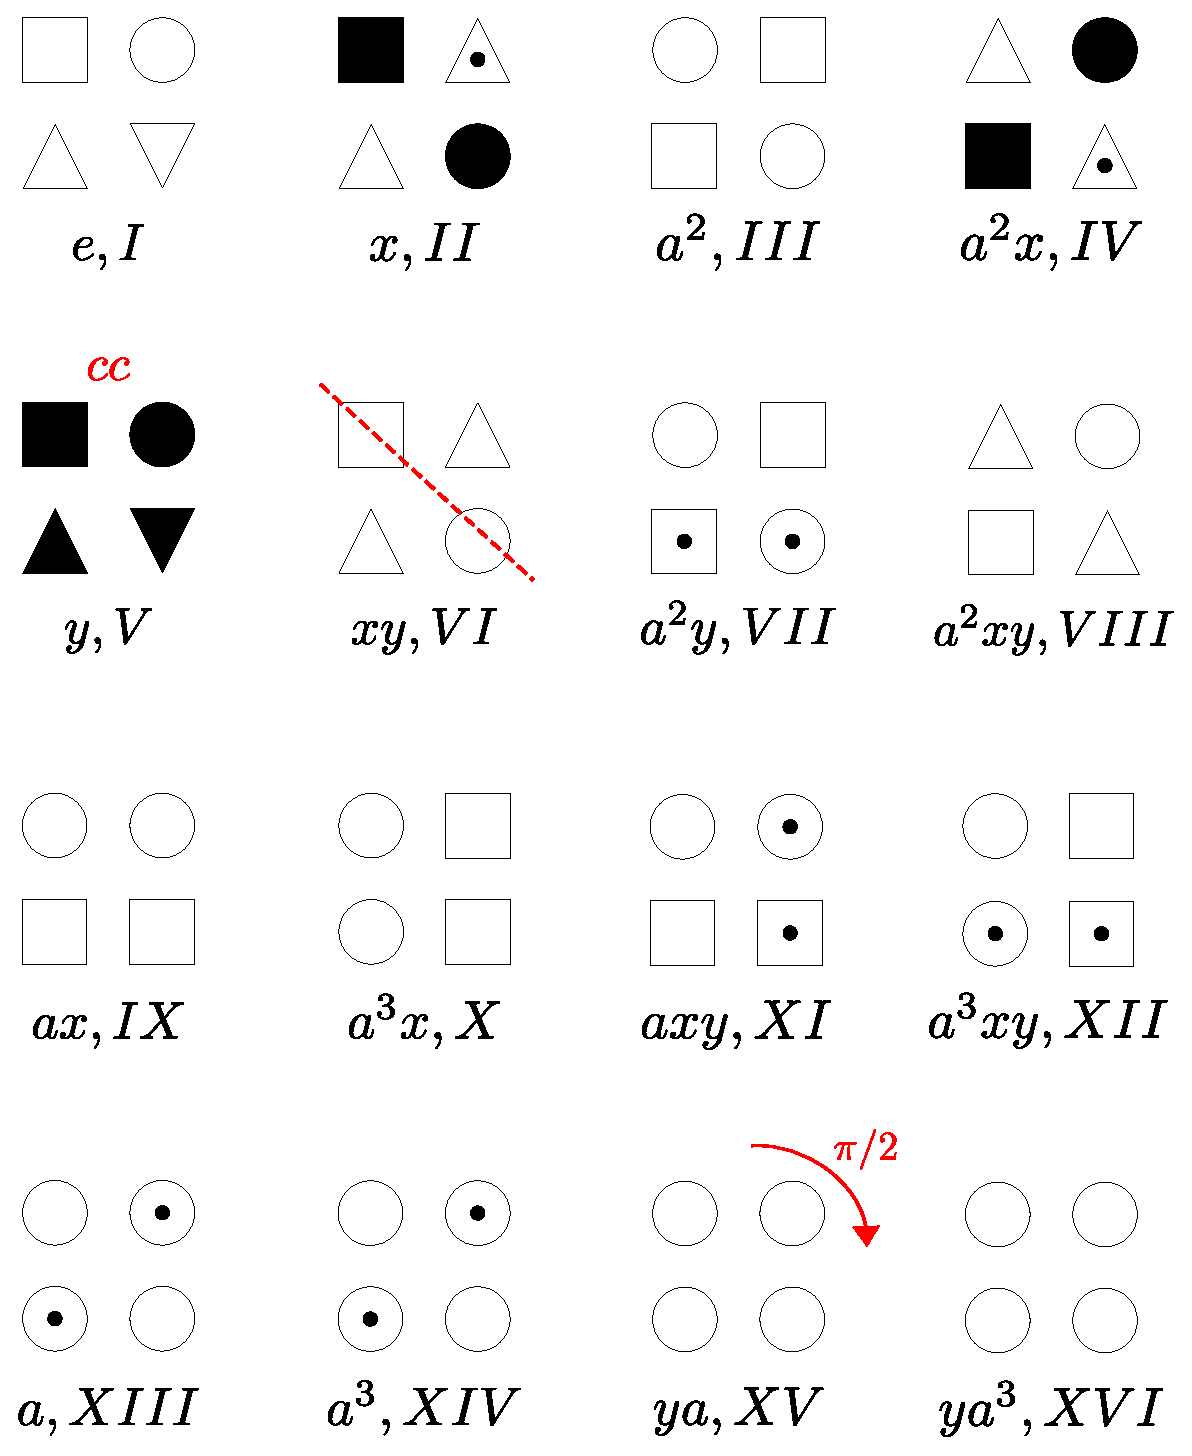
\includegraphics[width=75mm]{Figures/symmetries.eps}
\caption{Representation of $2\times2$ matrices  possesing the  sixteen symmetries compatible with $G_{16}$. The different symbols represent
different complex numbers. The dotted symbols are complex conjugate of undotted ones.  Filled symbols represent real
numbers. The roman number and group-theoretical codes are displayed below each matrix. All symmetry operations
can be constructed from three generators:  among different choices we may use $xy$ (flip along main diagonal), $y$ (complex conjugation), and $ya$ (rotation by $\pi/2$).}
\label{fig16}
\end{center}
\end{figure}
%%%%%%%%%%%%%%%%%


The reader may notice that the symmetries XIII and XIV are special in that they imply the same matrix structure,
as it also happens to
symmetries XV and XVI.
Here the distinction between symmetry operation and symmetry is quite crucial: Whereas
the symmetry operations XIII and XIV (or XV and XVI) are distinct, the corresponding symmetries
imply each other and hold under the same conditions for the matrix elements.  This special relation is explained in detail in the following section.

%\ref{inter}.
%

%%%%%%%%%%%%%%%%%%%%%%%%%%%%%%%%%%%%%%%%%%%%

\section{Implications of one or more  symmetries of the Hamiltonian \label{collapse}}

\subsection{Equivalence of symmetry operations and associated symmetries\label{secx}}
%
The  ``symmetries of $H$'' necessarily form a subgroup $G_{SH}$ with group structure, as the consecutive application of two
superoperators that leave $H$ invariant will also leave $H$ invariant.
This section explores the interplay between $G_{16}$ and $G_{SH}$, specifically the consequences of some existing symmetry. To that end we introduce two concepts: equivalent operations and associated symmetries.
%it is . Specifically An interesting feature of the group $G_{16}$ when realized as the set of operations on a Hamiltonian
%is the set of ``equivalences'' or ``associations'' of the symmetry operations
%which arise as a consequence on an existing symmetry or symmetries of $H$ represented by superoperators that leave $H$ invariant.


%, and we will show the effect of that in the form of equivalences between the other superoperators and associated symmetries.



We will say that,  {\it conditioned to  an existing symmetry or set of symmetries} \{${\cal S}_{i} H=H,
{\cal S}_{j}H=H, ...$\},
{two symmetry operations represented by ${\cal S}_k$  and ${\cal S}_l$ are {\bf equivalent},
${\cal S}_k\sim{\cal S}_l$ (more explicitly,  ${\cal S}_k\sim{\cal S}_l|\{{\cal S}_{i} H=H,
{\cal S}_{j}H=H, ...\}$)
if
${\cal S}_k H={\cal S}_l H$.}



${\cal S}_k\sim{\cal S}_l$  is indeed an equivalence relation in mathematical sense since it is
reflexive (a given superoperator is equivalent to itself); symmetric (if ${\cal S}_k\sim{\cal S}_l$, then
${\cal S}_l\sim{\cal S}_k$); and transitive (if ${\cal S}_k\sim{\cal S}_l$, and
${\cal S}_l\sim{\cal S}_m$, then ${\cal S}_k\sim{\cal S}_m$).



Equivalence relations provide partitions
 of the groups into  equivalence classes. In the $G_{16}$ group, each class is given by the superoperators that are equivalent to each other.   One of these classes is the group $G_{SH}$: All symmetry operations that leave the Hamiltonian invariant are equivalent among themselves and to the identity ${\cal L}_I$.


Equivalent pairs are easily found using the multiplication table of the group.  If ${\cal S}_i H=H$, then ${\cal S}_j={\cal S}_k {\cal S}_i$  (read from the table)
and ${\cal S}_k$  are equivalent.
%We emphasize that the equivalence ${\cal L}_\alpha\sim{\cal L}_\beta$ does not imply that the operations  represent necessarily symmetries of $H$, they may or may not. The equivalence states that the action of these two symmetry operations on $H$ gives the same result, that is all.

An example of equivalence that may be familiar to some
is that, conditioned on $xy H=H$ (which is satisfied in particular by all local potentials if we consider scattering
Hamiltonians in coordinate representation; more generally this symmetry implies that the matrix is complex-symmetric
or, equivalently, self-transpose),
then $a^2y H=a^2x H$. In the alternative operator language this means that, conditioned on $\theta H^\dagger\theta=H$,
we have that $\Pi\theta H\Pi \theta =\Pi H^\dagger \Pi$. In words, with the proper conditioning ($\theta$-pseudohermiticity, i.e., the symmetry of complex-symmetric matrices), the symmetry transformations related to PT-symmetry and to parity-pseudohermiticity give the same result when acting on the Hamiltonian. If it happens that
$H$ is indeed PT-symmetrical (i.e., $\Pi\theta H\Pi \theta=H$), then it will also be parity-pseudo-hermitian
($\Pi H^\dagger \Pi=H$)
and viceversa \cite{Mostafazadeh2010,Znojil2015}. These symmetry pairs  were explored systematically in \cite{Ruschhaupt2017} within the E8 group $\langle x,y,a^2\rangle$ studied  there, conditioned on a given (primary) symmetry. The novelty in the present work is twofold:  we
extend the analysis to $G_{16}$ and also define the equivalence relation more precisely, as a relation among symmetry operations acting on $H$:
as here defined, the equivalent pair is not necessarily a pair of Hamiltonian symmetries, but a pair of operations that, when acting on $H$, give the same result.









Two symmetry operations  represented by ${\cal S}_i$  and ${\cal S}_j$
are {\bf associated symmetry operations} if ${\cal S}_i\in G_{SH}\iff {\cal S}_j\in G_{SH}$.
%{\it and viceversa}.
In our group the two elements of order 4 in a given subgroup Z4 are associated symmetries:  $a$ and $a^3$ are associated, as well as $ay$ and $a^3y$.  The bidirectionality is important. For example $a\in G_{SH}\Rightarrow a^2\in G_{SH}$
but the reverse does not hold, so $a$ and $a^2$  are not associated symmetries.
Two associated symmetries imply the same structure on the Hamiltonian, i.e., the relations
that the matrix elements satisfy are equal in both cases, as illustrated in fig. \ref{fig16}.

Association is a stronger relation than equivalence since it  implies equivalence,
but equivalence does not imply association.

 %

%In prectic, we will specifically study the cases where one or two symmetries are assumed (the higher number of assumed symmetries will give us numerous special cases, but will not be useful to get general rules), and we will also give relevance to the rule generated for the general case (starting with the one symmetry case, to show a gradual development of the theory).

%This section relates closely to the previous one, since the origin of most of the relations  is the group structure of the set of superoperators.
% we will make a reasoning with the effects of this general properties, even so, we will accompany such reasonings with examples.
%Throughout the section it proves convenient to use a notation to label the superoperators which may differ
%from the one in Sec. \ref{sst}.

\subsubsection{Effects of one non-trivial symmetry of the Hamiltonian.}
%
%We will start by giving some simple examples of the more general cases we will study later.
For the following discussion some additional terminology is needed: A ``symmetry or order $n$'' represents the invariance of the Hamiltonian with respect to a superoperator of order $n$ (where $n$ is the minimal power $n\ge 1$ of the superoperator that gives  the identity).


{\it Symmetry of order 2.} Suppose that $H$ is invariant under $x$,  $xH=H$. Since $x^{2}=e$, the group composed by $x$ and $e$ is  in $G_{SH}$ (It might even be the full $G_{SH}$ if there are no other symmetries). Acting with $y$ on $x$ we have that
%and combine it with the members of the 2-group, we get the new superoperator $yx$($=xy$). Since $x$ and $yx$ commute, $yx$ and $y$ will be equivalent,
%
\begin{equation}
yx H=y(xH)=yH,
\end{equation}
%
so $yx\sim y$ conditioned on $xH=H$.
In fact there is nothing special about $y$ here. We can premultiply $x$ by the sixteen members of the group, to get
sixteen superoperators
${\cal S}_j x= {\cal S}_k$. If the index $j$ runs from $1$ to $16$, the index $k$ must jump among  the 16 members of the group
according to the multiplication table ($j\ne k$ except for $j=1$ assigned to the identity). Since $x$ is a symmetry of $H$,  ${\cal S}_k H={\cal S}_j H$, so that ${\cal S}_k\sim {\cal S}_j$ conditioned on $xH=H$.   It might seem that we have sixteen of these
equivalence pairs. However, multiplying ${\cal S}_j x= {\cal S}_k$ by $x$ from the right we find that ${\cal S}_j={\cal S}_k x$. This means that there are in fact only eight equivalence pairs; in other words, the relations (pairs of equivalent operations) are always repeated once.



The only property  of $x$ we have used, apart from representing a symmetry,
is $x^2=1$, so in general
{\it any symmetry of $H$ of order 2, implies eight pairs of equivalent superoperators}.  Conditioned on
$xH=H$,  in particular, we find the equivalences
%
\begin{eqnarray}
x\sim 1, ax\sim a, a^2x\sim a^2, a^3x\sim a^3,
\nonumber\\
ayx\sim ay, a^3yx\sim a^3y, yx^2\sim xy, a^2yx\sim a^2y.
\end{eqnarray}
%


{\it Symmetry of order 4.} Suppose now that $H$ is invariant under $a$ ($aH=H$). By applying $a$ repeatedly  we can create the subgroup of symmetries $\langle a \rangle$  in $G_{SH}$.
%(again it might be the full $G_{SH}$, we do not commit to one or  the other option by now).
Premultiplying the members of the group $\langle a \rangle$ by  $y$, we get the set of superoperators $ya,ya^{2},ya^{3},y$. They are all equivalent,
%
\begin{equation}
yH=y(aH)=yaH=ayH,
\end{equation}
\begin{equation}
yH=y(a^{2}H)=ya^{2}H=a^{2}yH,
\end{equation}
\begin{equation}
yH=y(a^{3}H)=ya^{3}H=a^{3}yH.
\end{equation}
%
The process may be repeated premultiplying the cyclic 4-group by $1$, $x$ and $xy$ instead of $y$. Let us recall that the full group
 of 16 elements may be constructed by multiplying the cyclic group $\langle a\rangle$ by $\langle x,y\rangle$.
Thus, this  premultiplication of $\langle a \rangle$ by the elements of $\langle x,y\rangle=\{1,x,y,xy\}$ gives
all 16 elements of the group $G_{16}$ without repetitions. Each member of $\langle x,y\rangle$ produces an equivalent class of 4 elements, namely,
%
\begin{eqnarray}
1,a,a^2,a^3,
\\
x,xa,xa^2,xa^3,
\\
y,ya,ya^2,ya^3,
\\
xy,xya,xya^2,xya^3.
\end{eqnarray}
%
The first set of 4 elements is formed by symmetries of $H$ while the others need not be symmetries.
Also, multiplication in reverse order, i.e., $\langle a\rangle \times \langle x,y\rangle$ produces exactly the same equivalence classes because of the property $xa=a^3 x$.



If $a^3$ is the assumed  symmetry of $H$
the same structure follows, since $a^3$ generates the same group of symmetries than $a$,
namely $\langle a\rangle=\langle a^3\rangle$.



When the  other elements of order 4, $ay$ and $a^3y$, are symmetries of $H$, they will also imply four sets of equivalent
superoperators,
%
\begin{eqnarray}
1,ay,a^2,ya^3,
\\
x,xay,xa^2,xya^3,
\\
y,y^2a,ya^2,a^3,
\\
xy,xa,xya^2,xa^3,
\end{eqnarray}
%
where, as before, the first set corresponds to symmetries of $H$. The others may or may not  be  symmetries of $H$.

\subsubsection{Consequences of two symmetries.}
%
Now suppose that the distinct superoperators  ${\cal S}_{i}$  and ${\cal S}_{j}$ represent two symmetries of $H$.
The consequences may be deduced by combining the results from the previous subsection.
Let us first recall that the two symmetries may generate groups of 2, 4, and 8 elements corresponding to symmetries as
discussed in the previous section.


- The case corresponding to groups of 2 elements is trivial as it requires that one of the symmetries
is the identity, and the other element should be of order 2.
Therefore the discussion of the consequences has already been done in the previous subsection.


In the following we assume that neither ${\cal S}_{i}$ nor ${\cal S}_{j}$ is the identity.



- A generated group of 4 elements $\langle {\cal S}_{i},{\cal S}_{j}\rangle$ corresponds to commuting operations except the combination of an element of order
4 and an element not in the cyclic groups $Z4$.  All elements of the generated group $\langle {\cal S}_{i},{\cal S}_{j}\rangle$ will be symmetries of $H$.
From there, the group table guarantees that it is always possible to find three other elements ${\cal S}_k$, ${\cal S}_l$, ${\cal S}_m$ such that the products
${\cal S}_{n}\langle {\cal S}_{i},{\cal S}_{j}\rangle$, where $n=k,l,m$, define three classes of equivalent operations. They are equivalent, respectively, to ${\cal S}_k$, ${\cal S}_l$, and ${\cal S}_m$.

Example:  ${\cal S}_{i}=x$;   ${\cal S}_{j}=y$. Then,
%
\begin{equation}
\langle {\cal S}_{i},{\cal S}_{j}\rangle=1,x,y,xy
\end{equation}
%
is a group of symmetries of $H$.
Choosing ${\cal S}_k=a$, ${\cal S}_l=a^2$, ${\cal S}_m=a^3$ we find  the three sets of equivalent operations
%
\begin{eqnarray}
a, ax, ay, axy
\nonumber\\
a^2,a^2x,a^2y,a^2xy
\nonumber\\
a^3,a^3x,a^3y,a^3xy
\end{eqnarray}
%


- Finally, when  $\langle {\cal S}_{i},{\cal S}_{j}\rangle$ has 8 elements, for example $\langle a,y\rangle$,
or $\langle x,a\rangle$, the eight elements are symmetries of $H$,
and {\it all other eight operations are equivalent to each other}. This is easy to prove. Multiplication of
any element ${\cal S}_k$ not in $\langle {\cal S}_{i},{\cal S}_{j}\rangle$ by the eight elements in $\langle {\cal S}_{i},{\cal S}_{j}\rangle$ must produce eight distinct elements not in $\langle {\cal S}_{i},{\cal S}_{j}\rangle$, because in the  group table each
element appears only once in any column (or row). These eight elements  are all equivalent to ${\cal S}_k$.
%If not such an element can be found it means that all elements are symmetries of $H$ and therefore (also) equivalent.
%
%
\subsubsection{Three or more symmetries.}
%
%
With three or more symmetries one may proceed similarly applying and combining the
results of the previous two subsections.
It is advisable to construct first the group generated by
the three superoperators of the symmetries. Several combinations  generate  directly the whole group of 16 elements,
for example $x$, $y$, and any element of order 4.  Other sets of 3 elements generate subgroups of 8 (for example
$\langle x,y,a^2\rangle$), or 4 elements (for example any three elements in a cyclic $Z4$ subgroup).
%
%
\section{Implications of the symmetries on the eigenvalues.\label{sp}}
%
%
If the Hamiltonian obeys a specific symmetry the eigenvectors and eigenvalues will fulfill certain conditions.
For example,  hermitian Hamiltonians imply real eigenvalues, and Hamiltonians that commute with
$\Pi$ will have even or odd eigenvectors.
A full and systematic analysis of the effect of all symmetries on the eigenvectors  is out of the scope of the present work
but we shall discuss here the
effect of the symmetries on the energy spectra because of its physical relevance.
%its completion is left as a pending question for future work. Nevertheless this point is obviously of much physical relevance
%so in this section we advance some important results and discuss several examples.


Let us first recall that the  symmetries for which eigenvalues come in conjugate pairs $E_j,E_j^*$
are symmetries II, IV, V, and VII, equivalently $x$, $a^2x$, $y$, and $a^2y$ in group-theory notation.
%This follows from theorems set by Ali Mostafazadehfazadeh, see e.g. \cite{Simon2019a},
%and corresponds to symmetries that can be expressed either as commutation of $H$ with an antilinear operator,
%or pseudohermiticity of $H$ with respect to some linear operator. T
The reason for having conjugate pairs has been well discussed,
see \cite{Mostafazadeh2002,Mostafazadeh2002a,Mostafazadeh2002b,Simon2019a}, so we shall not insist on it further, except for recalling that
the complex-pair condition implies the possibility to have real eigenvalues. While eigenvalues of Hermitian Hamiltonians $(xH=H)$
are always real, the reality of eigenvalues for symmetries $a^2x$, $y$,
and $a^2y$ is not guaranteed, and
requires specific parameter values, as discussed at length for PT-symmetry $(a^2yH=H)$  since the seminal work
\cite{Bender1998}.

%Some symmetries do not impose any particular relation or conditions  on the eigenvalues.
We shall next pay attention to implications on the eigenvalues of the symmetries of order 4 in the two cycles $Z4$.
% since they do have    implications on the eigenvalues.
For the other symmetries we have found no implications on the possible Hamiltonian eigenvalues, at least when they
are the only symmetries.
%
\subsubsection{$a, a^3$}
%
%
Let as assume that $aH=H$, or, explicitly, that $H=H^\dagger \Pi$.
Now we apply these operators on a right  eigenvector of $H$,
%
\begin{equation}
H|E\rangle=E|E\rangle=H^\dagger |\Pi E\rangle
\end{equation}
%
Acting with $\langle E|$ from the left in the last equality,
%
\begin{equation}
E\langle E|E\rangle=E^*\langle E|\Pi|E\rangle.
\label{condit}
\end{equation}
%
The matrix elements on both sides are real. Now we make use of the fact that
$a^2H=H$, or, translated into operators, $H=\Pi H\Pi$, i.e., $H$ commutes with $\Pi$.
%\Pi|E\rangle=\pm|E\rangle)$.
For right eigenvectors with even or odd parity we find that
%
\begin{eqnarray}
&&{\rm If}\;\; \Pi|E\rangle=|E\rangle \Rightarrow E\, {\rm is\, real},
\\
&&{\rm If}\;\; \Pi|E\rangle=-|E\rangle \Rightarrow E\, {\rm is\, imaginary}.
\end{eqnarray}
%
Of course the same splitting occurs when $a^3H=H$ since $a$ and $a^3$ are associated symmetries.
%
\subsubsection{$ay, a^3y$}
%
We now assume that $ayH=H$, i.e., $\theta H^\dagger\Pi\theta=H$. Note that, as before, $a^2 H=H$
holds as well automatically so that $H$ commutes with $\Pi$.
Making use of the ``diagonal'' biorthogonal  expression $H^\dagger=\sum |\widehat{E}\rangle  E^* \langle E|$
(we omit subindices) one finds, similarly to the previous calculation
%
\begin{equation}
E^*\langle E| \theta |E\rangle=E^*\langle E|\Pi|\theta E\rangle,
\end{equation}
%
which is now solved (assuming $\langle E| \theta |E\rangle\ne 0$)  according to the two possibilities
%
\begin{eqnarray}
&&{\rm If}\;\; \Pi|E\rangle=|E\rangle\Rightarrow   E\, {\rm is\, not\, restricted},
\\
&&{\rm If}\;\; \Pi|E\rangle=-|E\rangle \Rightarrow E=0,
\end{eqnarray}
%
The same result holds for the associated symmetry $a^3yH=H$.
%






\section{Discussion and conclusions\label{cd}}
%
In this work we have explored the symmetry operations on, and symmetries possessed
by, discrete (generally) non Hermitian Hamiltonians.
%\begin{itemize}
We have first seen that symmetry operations for discrete Hamiltonians are richer
that for scattering Hamiltonians because they are not restricted by the properties of the kinetic energy.
A non Abelian group of 16 symmetry operations arises naturally represented by linear and antilinear superoperators
that have geometrical interpretations
in terms of the symmetry operations of the square and complex conjugation.
A symmetry corresponds to the invariance of the Hamiltonian with respect to the transformation implied by one of these superoperators.
We have studied the properties and structure of this group and also
the implications of one or more existing symmetries in the rest of operations of the group,
introducing the  concepts of equivalent operations and of associated symmetries. The implications of some of these symmetries on the energy spectrum have also been discussed.
While some of these symmetries have been extensibly studied,  in particular PT-symmetry ($a^2yH=H$) \cite{Znojil2015}, complex symmetric matrices ($xyH=H$) \cite{Garcia2014},
and of course hermitian matrices ($xH=H)$, the broader frame introduced in this work provides a basis to relate,
understand and exploit multiple symmetries and their interconnections.
Combining discrete and continuous symmetry operations is also possible, as in \cite{Kartashov2014,Zezyulin2017}.






%\end{itemize}

Some open questions and ideas for future work are:
i) To set the relation with optical systems or quantum optical systems and develop
applications such as finding selection rules or device engineering.
In particular physical realizations of non-hermitian symmetries different from $PT$, e.g. with respect to
$a^2$, $xy$, $a^2xy$, are doable
in a quantum optical setting using two-level atoms interacting with a laser beam \cite{Ruschhaupt2004a}.
Our emphasis has been on Hamiltonians but general complex matrices of physical interest, such as  a characteristic matrix of a stratified medium \cite{Born1964},
are of course amenable to be transformed by operations in  $G_{16}$ and may posses some of the
implied symmetries, e.g. with respect to $a$ or $a^3$; ii) To complete a systematic study of the effect of the 16 symmetries on right/left eigenvectors; iii)  To work out a ``representation theory'' for non Hermitian symmetries; iv) To extend the symmetries further. For example the symmetries described have their ``negative'' versions
in the form ${\cal S}H=-H$, or even more generally ${\cal S}H= e^{i\phi} H$, with $\phi$ being a real phase. In this regard it would be very interesting to relate the present work to the Bernard-LeClair symmetry classes
of non-Hermitian random matrices and their variants \cite{Bernard2002, Kawabata2019}. We just note at this point that
some of the symmetries implied by $G_{16}$ are not of the forms considered in $\cite{Bernard2002}$.
